\chapter{Relations between perfusion parameters: theoretical and experimental considerations}\label{chapter:PMB2}
\section{Introduction}
This chapter is a complement to the work presented in Chapter~\ref{chapter:PMB}, and relies on the same experimental data, mathematical models, and notations.
It aims at establishing the relations between the semi-quantitative perfusion parameters commonly derived from the Log-Normal model, and the relations between these parameters and the quantitative parameters of the one-compartment model.
The relations between parameters were first established theoretically, and then experimentally through correlation studies.

\section{Theory}
This section gives the closed-form expressions of $AUC$, $PE$, $TTP$, $MTT$, $WIR$, $WOR$, and $TD$ parameters for the Log-Normal model, \textbf{aLN} (Table \ref{tab:AnalyticRelation}), and for the one-compartment model, \textbf{aAIFd} (Table \ref{tab:AnalyticRelationAIF}).
The equations of the models are given in Section~\ref{sec:models} of Chapter~\ref{chapter:PMB}.

$AUC$ was defined as the infinite integral of the function, $PE$ as the value taken by the function where its derivative is null, $TTP$ the time where the function derivative is null, $MTT$ as the expected value of the function normalized by its $AUC$, the $WIR$ and $WOR$ as the derivative of the function where its second order derivative is null, and $TD$ as the time-delay of the function.

\begin{table}[!h]
\begin{center}
\begin{tabular}{lc}
\toprule
\textbf{$AUC$} & $A$ \\
\midrule
\textbf{$TTP$} & $e^{\mu - \sigma^2}$  \\
\midrule
\textbf{$PE$} & $A\frac{e^{\frac{\sigma^2}{2}-\mu}}{\sigma \sqrt{2\pi}}$  \\
\midrule
\textbf{$MTT$} & $e^{\mu + \frac{\sigma^2}{2}}$ \\
\midrule
\textbf{$WIR$}
 & $\frac{A}{\sigma\sqrt{2\pi}}\left(\frac{y}{\sigma^2}-1\right)e^{2y-2\mu-\frac{y^2}{2\sigma^2}}$, where $y = \frac{3\sigma^2+\sigma\sqrt{\sigma^2+4}}{2}$ \\
\midrule
\textbf{$WOR$} & $\frac{A}{\sigma\sqrt{2\pi}}\left(1-\frac{z}{\sigma^2}\right)e^{2z-2\mu-\frac{z^2}{2\sigma^2}}$, where $z = \frac{3\sigma^2-\sigma\sqrt{\sigma^2+4}}{2}$ \\
\midrule
\textbf{$TD$} & $\Delta_T$ \\
\bottomrule
\end{tabular}
\caption{Closed-form expressions of perfusion parameters using the \textbf{aLN} model, WOR being the absolute value of the maximum negative slope.}
\label{tab:AnalyticRelation}
\end{center}
\end{table}

\begin{table}[!h]
\begin{center}
\begin{tabular}{lccc}
\toprule
AIF & \textbf{$K\delta\left(t\right)$} & $K rect_a\left(t\right)$ & $C_A \left(t\right)$ \\
\midrule
\textbf{$AUC$} & $KV_T$ & $KV_T$ & $V_T \int_{0}^{+\infty}C_A\left(\tau\right)\mathrm d\tau$\\
\midrule
\textbf{$TTP$} & 0  & $a$ & $\{ t_P \enskip\vert\enskip C_T\left(t_P - d_T\right) = V_T C_A\left(t_P \right)\}$ \\
\midrule
\textbf{$PE$} &  $KF_T$ & $\frac{KV_T}{a}\left(1-e^{-\frac{aF_T}{V_T}}\right)$ & $F_Te^{-\frac{F_T}{V_T} t_P}\int_{0}^{t_P}C_A\left(\tau\right)e^{\frac{F_T}{V_T} \tau}\mathrm d\tau$ \\
\midrule
\textbf{$MTT$} & $\frac{V_T}{F_T}$ & $\frac{V_T}{F_T} + \frac{a}{2}$ & $\frac{V_T}{F_T} + MTT_{C_A}$ \\
\midrule
\multirow{2}{*}{\textbf{$WIR$}}
 &  \multirow{2}{*}{$\infty$} & \multirow{2}{*}{{$\frac{KF_T}{a}$}} & $F_T\left(C_A\left(t_{I}\right)-\frac{1}{V_T}C_T\left(t_{I} - d_T\right)\right)$ \\
&  & & $\{ t_{I} \enskip\vert\enskip \frac{\mathrm d C_T}{\mathrm dt}\left(t_{I} - d_T\right) = V_T \frac{\mathrm d C_A}{\mathrm dt}\left(t_{I}\right), \frac{\mathrm d C_A}{\mathrm d t}\left(t_{I}\right) > 0\}$ \\
\midrule
\multirow{2}{*}{$WOR$} &  \multirow{2}{*}{$\frac{KF_T^2}{V_T}$} & \multirow{2}{*}{$\frac{KF_T}{a}\left( 1-e^{-\frac{aF_T}{V_T}} \right)$} & $F_T\left(C_A\left(t_{O}\right)-\frac{1}{V_T}C_T\left(t_{O} - d_T\right)\right)$ \\
& & & $\{ t_{O} \enskip\vert\enskip \frac{\mathrm d C_T}{\mathrm d t}\left(t_{O} - d_T\right) = V_T \frac{\mathrm d C_A}{\mathrm d t}\left(t_{O}\right),\frac{\mathrm d C_A}{\mathrm d t}\left(t_{O}\right) < 0\}$ \\
\midrule
$TD$ & $d_T$ & $d_T$ & $d_T$ \\
\bottomrule
\end{tabular}
\caption{Closed-form expressions of perfusion parameters using a one-compartment model (\textbf{aAIFd}) and assuming three different shapes of AIF: impulse function $(\delta)$, rectangle function of width $a$ and height $1/a$, $rect_a(t)$, and general case $C_A(t)$. In the first two cases, $K$ stands for the injected concentration. In the general case, $MTT_{C_A}$ stands for the mean transit time of $C_A(t)$.}
\label{tab:AnalyticRelationAIF}
\end{center}
\end{table}

\begin{table}[!h]
\begin{center}
\begin{tabular}{lccc}
\toprule
AIF & \textbf{$K\delta\left(t\right)$} & $K rect_a\left(t\right)$ & $C_A \left(t\right)$ \\
\midrule
\textbf{$rAUC$} & $\frac{V_T}{V_R}$ & $\frac{V_T}{V_R}$ & $\frac{V_T}{V_R}$\\
\midrule
\multirow{3}{*}{\textbf{$rWIR$}} &  \multirow{3}{*}{--} & \multirow{3}{*}{{$\frac{F_T}{F_R}$}} & $\frac{F_T\left(C_A\left(t_{I,T}\right)-\frac{1}{V_T}C_T\left(t_{I,T} - d_T\right)\right)}{F_R\left(C_A\left(t_{I,R}\right)-\frac{1}{V_R}C_R\left(t_{I,R} - d_R\right)\right)}$ \\
&  & & $\{ t_{I,T} \enskip\vert\enskip \frac{\mathrm d C_T}{\mathrm dt}\left(t_{I,T} - d_T\right) = V_T \frac{\mathrm d C_A}{\mathrm dt}\left(t_{I,T}\right), \frac{\mathrm d C_A}{\mathrm d t}\left(t_{I,T}\right) > 0\}$ \\
&  & & $\{ t_{I,R} \enskip\vert\enskip \frac{\mathrm d C_R}{\mathrm dt}\left(t_{I,R} - d_R\right) = V_R \frac{\mathrm d C_A}{\mathrm dt}\left(t_{I,R}\right), \frac{\mathrm d C_A}{\mathrm d t}\left(t_{I,R}\right) > 0\}$ \\
\midrule
$rTD$ & $d_T - d_R$ & $d_T - d_R$ & $d_T - d_R$ \\
\bottomrule
\end{tabular}
\caption{Closed-form expressions of the relative perfusion parameters using a relative one-compartment model (\textbf{rAIFd}) and assuming three different shapes of AIF: impulse  function $(\delta)$, rectangle function of width $a$ and height $1/a$, $rect_a(t)$, and general case $C_A(t)$. In the first two cases, $K$ stands for the injected concentration.}
\label{tab:AnalyticRelationRelative}
\end{center}
\end{table}

\section{Data Analysis}
Coefficients of determination $R^2_{\theta_{i},\theta_{j}}$ were estimated from the least-squares linear regression between the 32 regional estimates of parameters $\theta_{i}^{h}$ and $\theta_{j}^{h}$, one estimate per sub-region $s_{h})$. These coefficients were computed independently for each of the 16 DCE-US studies (4 mice $m_{l}$ $\times$ 4 test-restest studies $R_{k}$). A linear regression was also computed between sets of $512$ parameters (the 32 sub-regions of the 16 studies were polled together) to assess the consistency of the relationships between parameters. 

\section{Results}
\begin{figure}[ht]
  \centering
  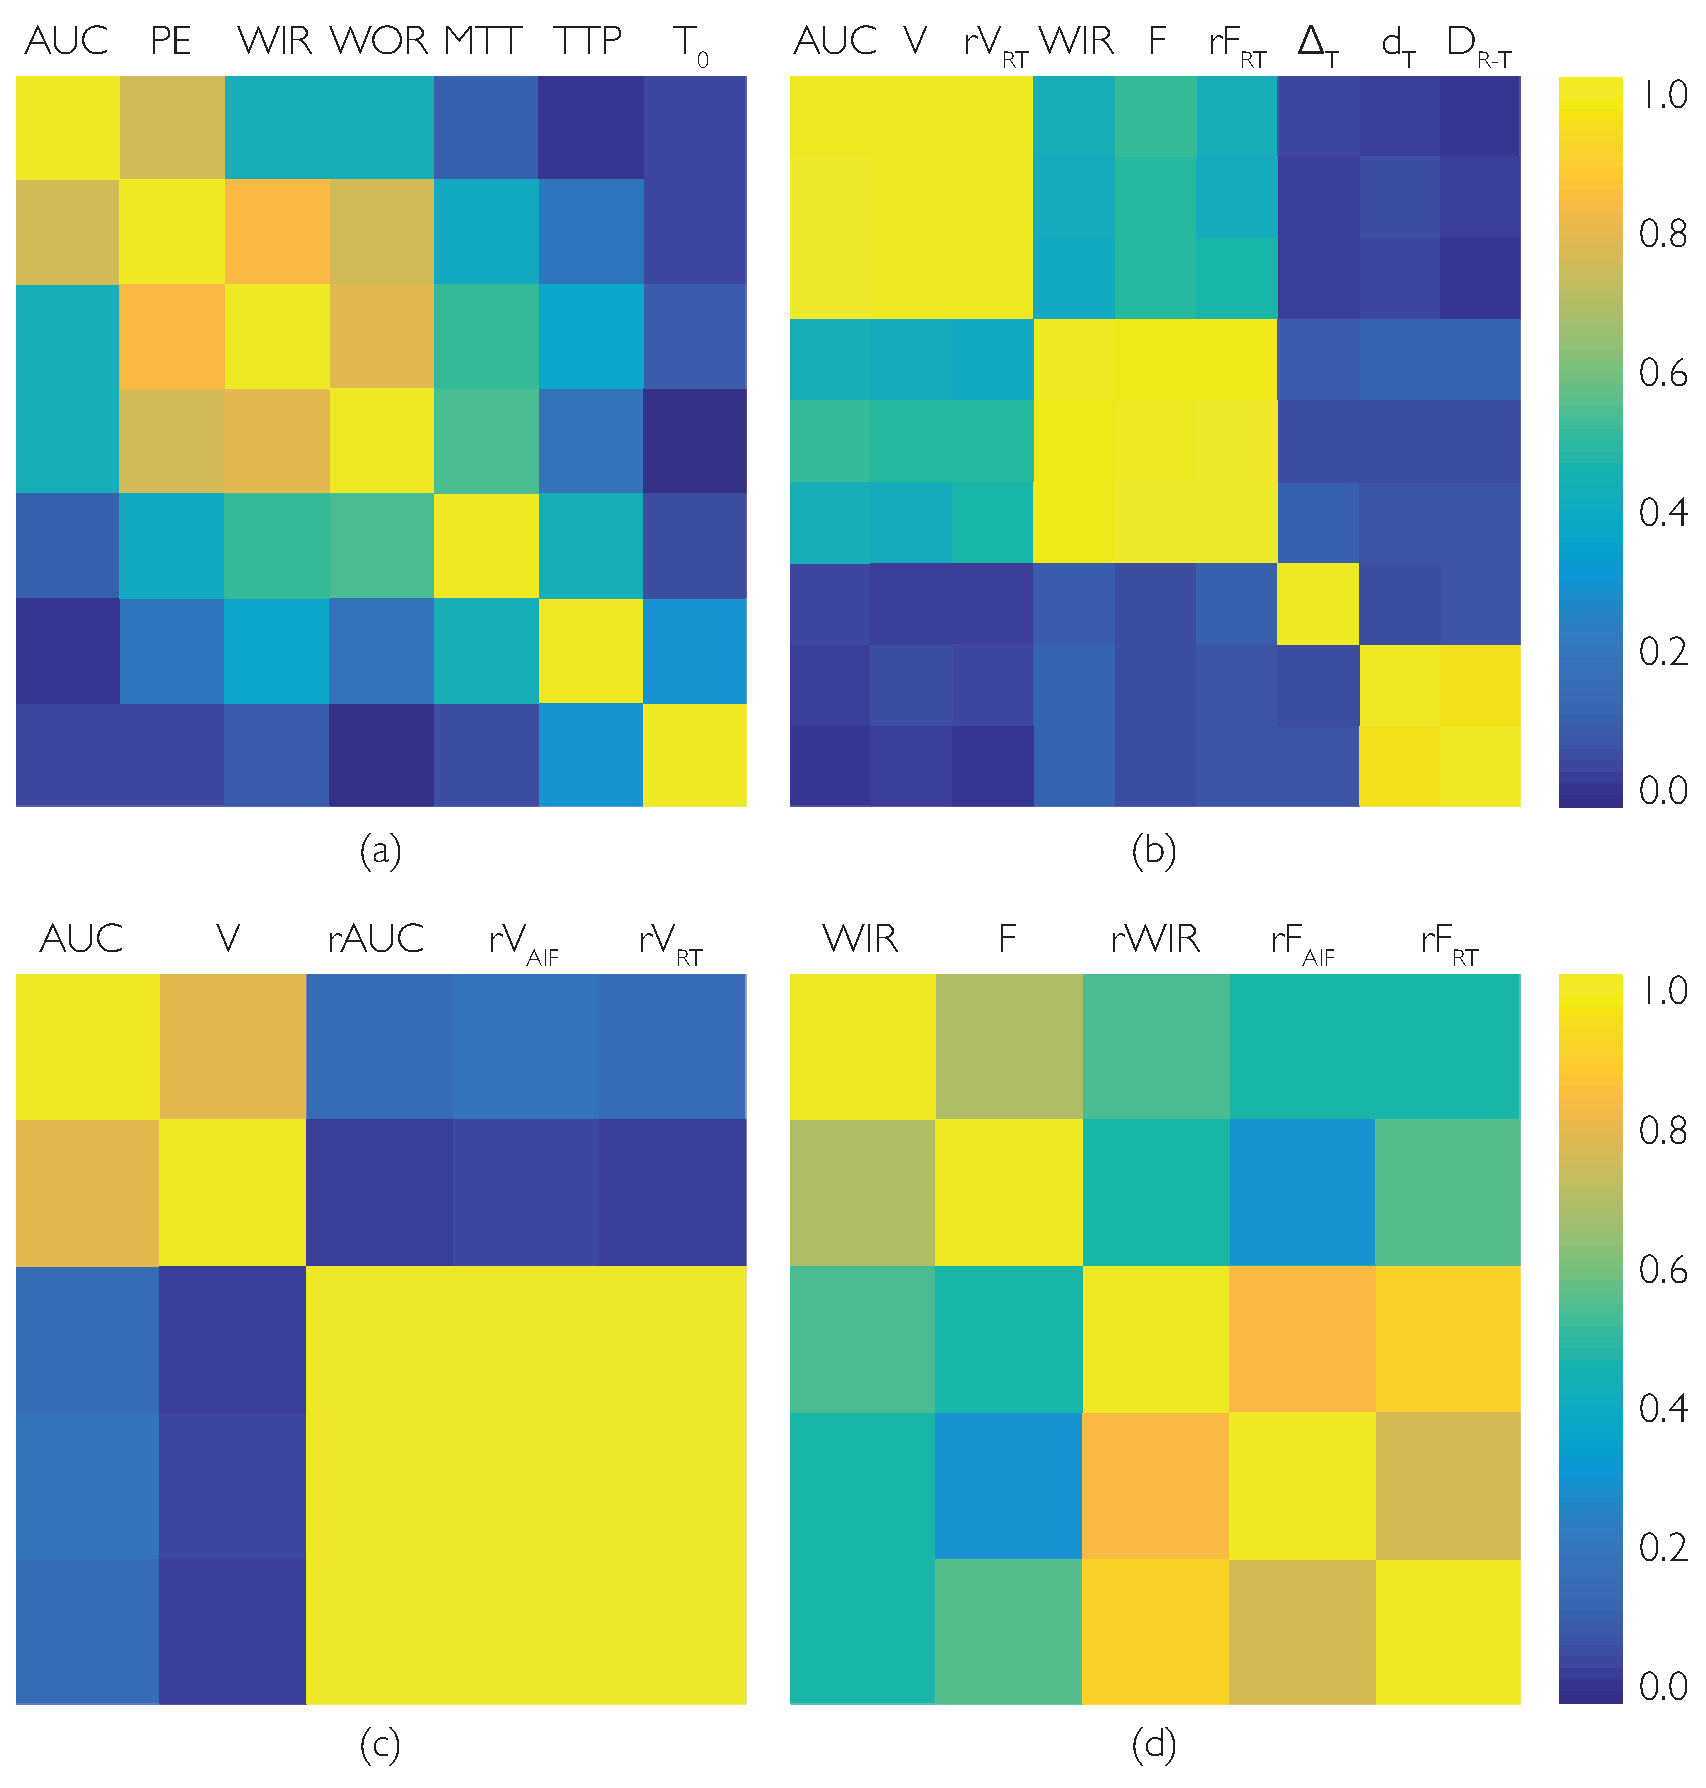
\includegraphics[width=\linewidth]{R2HeatMap.eps}
  \caption{(a-b) Median (of $16$ values) coefficient of determination ($R^2$) of the least-squares linear regression between pairs of parameters $\left(\theta_i, \theta_j\right)$ computed for the 32 sub-regions of one exam: (a)~parameters derived from the \textbf{aLN} approach; (b)~volume ($AUC$, $V$ and $rV_{RT}$), flow ($WIR$, $F$ and $rF_{RT}$) and time delay ($\Delta_T$ , $d_t$ and $D_{RT}$) parameters respectively computed with \textbf{aLN}, \textbf{aAIFd}  and \textbf{RTd} models. (c-d) Coefficients of determination ($R^2$) of the least-squares linear regression computed when pooling the 512 sub-regions  together: (c) $R^2$ between pairs of volume parameters computed with \textbf{aLN}, \textbf{aAIFd}, \textbf{rLN}, \textbf{rAIFd}  and \textbf{RTd} models, (d) $R^2$ between pairs of flow parameters computed with \textbf{aLN}, \textbf{aAIFd}, \textbf{rLN}, \textbf{rAIFd} and \textbf{RTd} models.}
  \label{fig:R2HeatMaps}
\end{figure}

The heatmaps shown in Figure~\ref{fig:R2HeatMaps} correspond to $R^2_{\theta_{i}\theta_{j}}$ coefficients from the linear regressions between pairs of parameters $\left(\theta_{i}, \theta_{j}\right)$. Figure~\ref{fig:R2HeatMaps}~(a) shows the $R^2$ coefficients between all pairs of parameters derived from the \textbf{aLN} model. It reveals strong linear relationships between some of the parameters, especially $\mathrm{median}\left(R^2_{AUC, PE}\right)$, $\mathrm{median}\left(R^2_{PE, WIR}\right)$, $\mathrm{median}\left(R^2_{WIR, WOR}\right)$. The formal non-linear relationships between these parameters (expressed in Table~\ref{tab:AnalyticRelation}) generate high linear links and thus information redundancy. For that reason we further focused on three derived parameters: $AUC$, which is related to tissue blood volume $V$, according to the closed-form expressions given in Table~\ref{tab:AnalyticRelationAIF}, $WIR$, which is mainly related to tissue blood flow $F$), and the delay parameter $\Delta$. In addition, Table~\ref{tab:AnalyticRelationRelative} shows the formal relations between the relative value of $AUC$ ($rAUC$) and $WIR$ ($rWIR$) and the parameters of the \textbf{aAIFd} model. It reveals that $rAUC$ and $rV$ are equivalent, and that $rWIR$ is linearly related to $rF$ in the general case of input function, the proportionality coefficient depending on $C_A\left(t\right)$. These theoretical identifications were confirmed experimentally by Figure~\ref{fig:R2HeatMaps}~(b) which shows strong linear relationships between volume (first 3 rows/columns) and flow parameters (middle 3 rows/columns). For instance, the linear regressions between $AUC$, $V$ and $rV_{RT}$ all yielded median $R^2$ values greater than $0.95$. The same trend is observed for $WIR$, $F$ and $rF_{RT}$. The correlations between volume parameters and flow parameters are medium ($\mathrm{median}\left(R^2_{V, F}\right) < 0.50$). Finally for the time parameters (last 3 rows/columns), there is a high correlation between $d$ and $D$ but there is no correlation between $\Delta$ and the other time delays ($\mathrm{median}\left(R^2\right) < 0.15$). 

Figure~\ref{fig:R2HeatMaps}~(c) and Figure~\ref{fig:R2HeatMaps}~(d) show the trends observed on flow and volume parameters when pooling parameters issued from all the exams. 
There is a very high correlation ($R^2 > 0.95$) between the relative volume parameters $rAUC$, $rV_{AIF}$, and $rV_{RT}$ and a high correlation ($R^2 > 0.75$) between the relative flow parameters $rWIR$, $rF_{AIF}$, and $rF_{RT}$. Correlations are poor ($R^2 < 0.20$) between absolute and relative volume parameters, and medium between absolute and relative flow parameters ($R^2< 0.55$). Since the intra-exam correlations between volume (resp.~flow) parameters are high, the correlation over pooled data reflects the inter-exam consistency of linear regression slopes: it is much higher for relative volumes (or flows) than for absolute volumes (or flows). Figure \ref{fig:Slopes} from Chapter~\ref{chapter:PMB} illustrates this trend for one specific mouse ($m_1$). 
\FloatBarrier


\section{Discussion}
The equations given in Table~\ref{tab:AnalyticRelation} were used in Chapter~\ref{chapter:PMB}, and later in this thesis, to analytically derive the perfusion parameter values from the fitted Log-Normal model, therefore avoiding numerical approximations.

Interestingly, Figure~\ref{fig:R2HeatMaps} reveals strong correlations between the parameters estimated by the various approaches, however Figure~\ref{fig:Slopes} shows large variations of the regression slopes between exams. Thus all the parameters can be used to assess spatial tumor heterogeneity. However, when it comes to the comparison of longitudinal exams, it is crucial to have comparable parameter values. Thus, relative parameters seem to be the most powerful solution, provided that the reference tissue can be defined in each exam, and that its characteristics are not modified between successive exams.

Some studies stated that $AUC$ is related to tissue blood flow, this theoretical and experimental study demonstrates its relation to tissue blood volume instead.

\section{Conclusion}
A comprehensive comparison of the parameters estimated by different approaches was proposed, showing high correlations between the volume-based and flow-based parameters respectively estimated.